\chapter[Estado del Arte]{Estado del Arte}
\label{cp:state-of-the-art}

En este capítulo se presentan los conceptos teóricos y los proyectos científicos en los que se apoya este trabajo. Para entender cómo una 
inteligencia artificial puede clasificar los usos del suelo en las imágenes de manera autónoma, primero tenemos que ver qué estándares se 
usan hoy en día en la comunidad científica, cómo funcionan los satélites que nos envían las imágenes, cómo se gestionan las coordenadas 
geográficas en los mapas y, por último, cómo funcionan por dentro las redes neuronales que procesan estos datos. Para obtener la información
hemos hecho uso del buscador de Google buscando palabras claves como "Sentinel-2" o "BigEarthNet". Nos hemos centrado en la información 
relevante que define nuestro problema. 

\section{Conceptos de Teledetección y satélites: La misión Sentinel-2}
\label{sentinel_2}

La teledetección permite obtener información de la superficie terrestre a distancia, sin necesidad de entrar en contacto con ella. Lo cual se 
consigue midiendo la radiación electromagnética que los diferentes elementos en la Tierra (como el agua, la vegetación o carreteras) reflejan
cuando los ilumina el Sol. Cada superficie interactúa con la luz de maneras únicas según sus propiedades, haciendo que absorba unas longitudes
de onda más y otras menos, lo que genera lo que se conoce como firma espectral, la cual recogen los satélites que usamos en este proyecto (Sentinel-2).


Como se ha mencionado previamente, los datos han sido extraídos de la misión Copernicus Sentinel-2, la cual consiste en 2 satélites colocados
en extremos opuestos de la Tierra (S-2B y S-2C) y uno operando temporalmente a 36º de S-2B (S-2A), con una franja de obtención de datos de 290 
kilómetros y un periodo bajo para la actualzación de los datos, permitiendo la monitorización de los cambios sobre la superficie de la Tierra.
Estos datos están a disposición del público general de manera gratuita por parte de la \acrfull{esa}. Estos satélites disponen de un sensor
óptico que permite capturar 13 bandas espectrales con distintos niveles de resolución espacial (10, 20 y 60 metros por píxel), distriibuidas a 
lo largo del espectro visible e infrarrojo, tanto cercano (NIR), como de onda corta (SWIR), como se puede ver en la Figura \autoref{fig:bandas} \cite{dataspace.copernicus.eu}.

\begin{figure}[!htpb]
    \centering
    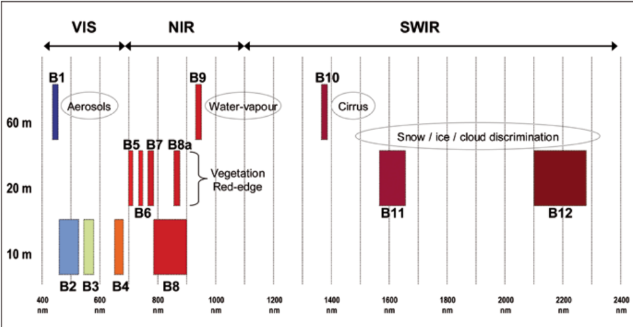
\includegraphics[width=0.5\linewidth]{Img/Theme/bandasSentinel2.png}
    \caption[Registro espectral de Sentinel-2]{Imágen con las 13 bandas espectrales que recoge Sentinel-2 y sus respectivas resoluciones espaciales\cite{cursosteledeteccion.com}}
    \label{fig:bandas}
\end{figure}

Para no usar tantos recursos a la hora de procesar las imágenes, en este trabajo tan solo nos quedamos con las bandas asociadas a una resolución 
de 10 metros por píxel, dándonos el mayor nivel de detalle sobre el terreno, buscando un equilibrio entre eficiencia y precisión, manteniendo
las bandas B02, B03, B04 y B08. Las 3 primeras bandas son las encargadas del espectro visible, azul, verde y rojo respectivamente, y la última
se encarga del \acrfull{nir}, las cuales recogen los valores de reflectancia de la superficie terrestre para cada uno de los cuatro espectros. 
Usando así solo estos 4 canales, buscamos una información geométrica y espectral óptima sin saturar la memoria del ordenador.

\section{Cartografía y \acrfull{crs}}
\label{ccrs}

Para que los datos sean útiles es necesario cuadrar exactamente las imágenes satelitales con el mapa de uso de suelo real. Para ello es necesario
tener un \acrfull{crs} definido. En cartografía, es necesario representar un objeto tridimensional en una superficie bidimensional, surge
la necesidad de un \acrshort{crs} y un sistema de proyecciones es usado para el almacenamiento e interpretación de los datos.


El primer concepto clave es el \acrlong{etrs} 1989 (\acrshort{etrs}89). Es el marco oficial de referencia de la Unión Europea para toda la 
cartografía pública, y al situarse sobre la placa euroasiática, la cual es estática bajo este marco, no están sujetos a cambios debido a los 
movimientos de las placas, lo que aporta una estabilidad a nuestros mapas \cite{wikipedia.etrs89}.


El segundo concepto es la \acrfull{utm}. Al ser la Tierra redonda y surgir la necesidad de representarla sobre superficies planas, es necesaria
una proyección que transforme el sistema esférico, de latitud y longitud, ignorando la altitud, en metros reales (ejes X e Y). Esta proyección se encarga de dividir 
el planeta en 60 zonas llamadas "husos", que se expanden normalmente por 6º de la esfera terrestre, buscando así la mínima distorsión provocada
por la curvatura de la misma. Bajo este sistema de proyección España cae principalmente en los husos 29, 30 y 31.\cite{wikipedia.utm}


Para unificar los 2 sistemas anteriores, se creó un estándar internacional llamado \acrfull{epsg}, el cual tiene asociado  tanto un \acrshort{crs}
como un huso \acrshort{utm}. En nuestro caso nos interesaba el \acrshort{epsg}:25830, el cual representa el marco europeo y la proyección sobre 
el huso 30 de manera unificada. De esta forma, si aseguramos que todos nuestros datos están en el estándar \acrshort{epsg}:25830, garantizamos
que las imágenes del Sentinel-2 y el mapa con las etiquetas de la covertura del suelo se alineen perfectamente \cite{epsgwiki}.

\section{Cartografía oficial de ocupación del suelo: CORINE y SIOSE}
\label{etiquetas_suelo}

Para entender de dónde proceden las etiquetas de entrenamiento de nuestro modelo, es necesario analizar los estándares oficiales de ocupación del suelo.
A nivel de España encontramos dos principales:


El programa \acrfull{clc} surge como "Un proyecto experiemntal para la recopilación de datos, la coordinación y la homogeneización
de la información sobre el estado del Medio Ambiente y los recursos naturales de la Comunidad" según \cite{corinelandcover}. Se caracteriza por
disponer de una información homogénea para toda Europa, la suficiente información para la toma de decisiones que son afectadas por estos cambios 
en el medio ambiente a nivel europeo. Dispone de 5 versiones distintas tomadas en 1990, 2000, 2006, 2012 y 2018, con el fin de ir actualizándolo
de manera periódica cada seis años a una escala de 1:100000.


La cobertura ofrecida por \acrshort{clc} tiene una resolución de 25 hectáreas de manera general y de 5 hectáreas para zonas que 
hayan sufrido cambios entre versiones, con el fin de representar de manera más precisa estos cambios. Independientemente de esto, cabe resaltar
como la resolución de 25 hectáreas es justo equivalente a nuestros bloques de $50\times 50$ píxeles a resolución de 10 metros por píxel.


Con el fin de clasificar de la forma mas precisa la cobertura del suelo, \acrshort{clc} contiene 44 clases con 3 niveles de detalle como se puede
ver en las Figuras \autoref{label} y \autoref{label}.

\begin{figure}[!htpb]
    \centering
    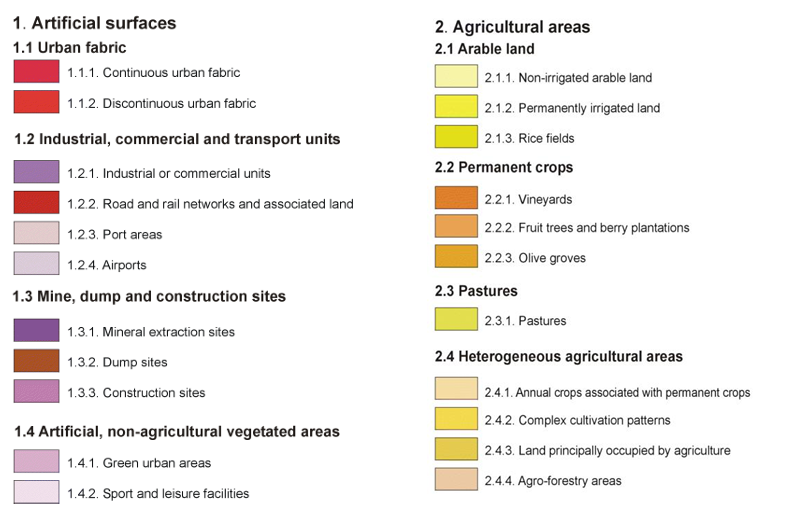
\includegraphics[width=0.5\linewidth]{Img/Theme/clc1.png}
    \caption[Primera parte clasificación CLC]{Nomenclatura de 3 niveles \acrshort{clc} \cite{corinelandcover}}
    \label{fig:clc1}
\end{figure}
\begin{figure}[!htpb]
    \centering
    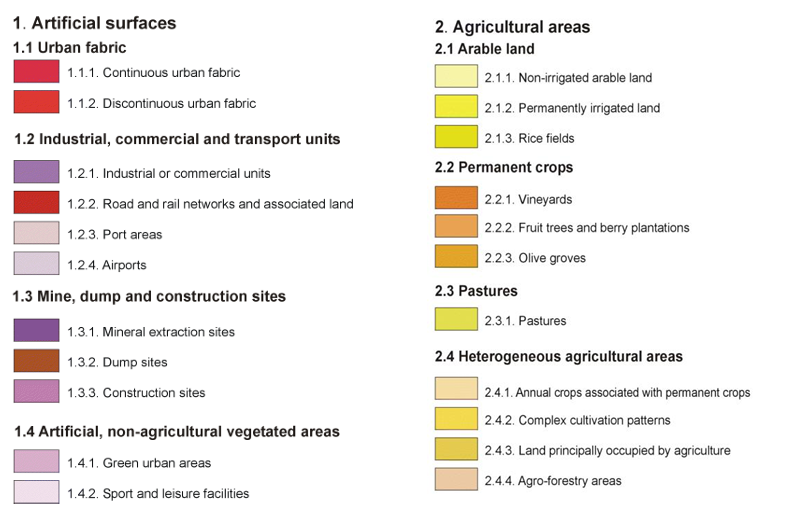
\includegraphics[width=0.5\linewidth]{Img/Theme/clc1.png}
    \caption[Segunda parte clasificación CLC]{Nomenclatura de 3 niveles \acrshort{clc} \cite{corinelandcover}}
    \label{fig:clc2}
\end{figure}


Además de \acrshort{clc}, en España también existe el proyecto \acrfull{siose}, el cual trabaja con una escala nominal de 1:25000 (cuatro veces 
más detallada que \acrshort{clc}) para los años 2005, 2009, 2011 y 2014 a nivel de Comunidad Autónoma \cite{sioseb}. Actualmente, este proyecto tradicional no 
está en producción, dando paso a \acrshort{siose} de Alta Resolución (SIOSE-AR), el cual mejora entre 5 y 25 veces la escala de su versión 
antigua, moviéndose en rangos de 1:1000 a 1:5000 \cite{siosear}.

\section{El estándar de referencia BigEarthNet}
\label{bigearthnet}

Gracias a los avances en el aprendizaje profundo, el análisis de imágenes de satélite ha dado un gran salto debido a la capacidad de las
redes neuronales para entender el contenido visual de forma automática. Sin embargo, para entrenar estos modelos se necesitan una cantidad masiva
de imágenes etiquetadas, algo que durante mucho tiempo ha supuesto un cuello de botella en este sector. La mayoría de las bases de datos antiguas 
eran pequeñas o clasificaban cada foto con una etiqueta global, ignorando que en una imagen de satélite pueda haber varios tipos de suelo simultáneamente 
\cite{bigearthnet}.


Para resolver este problema, la Universidad Técnica de Berlín creó \textbf{BigEarhNet}, un conjunto de datos diseñado específicamente como fuente
de entrenamiento para modelos de inteligencia artificial, a partir de 125 macroparches entre junio de 2017 y mayo de 2018. A nivel científico, este 
estándar reúne imágenes de la misión Sentinel-2 (con menos de un 1\% de nubes) y las divide en casi 600000 parches independientes. Cada uno de 
estos parches funciona como una matriz de dimensiones fijas, 
y varía su tamaño en función de la de la banda usada del satélite: \begin{itemize}
    \item Las bandas de 10 metros de resolución se recortaron en una matriz de $120\times 120$ píxeles
    \item Las bandas de 20 metros de resolución se recortaron en una matriz de $60\times 60$ píxeles
    \item Las bandas de 60 metros de resolución se recortaron en una matriz de $20\times 20$ píxeles
\end{itemize}

La gran ventaja de usar BigEarthNet como molde para este proyecto es que usan etiquetas de \acrshort{clc}, y además llegan a la conclusión de
que las 44 clases pueden reducirse a tan solo 19 clases, consiguiendo mayor estabilidad en los modelos, también eliminan parches con gran porcentaje 
de nubes o nieve antes de empezar el entrenamiento.


Como las versiones de este estándar se actualizan de manera constante, basar nuestro trabajo en su estructura nos permite tener la certeza
de que el TFG sigue los estándares científicos actuales. En nuestro caso, adaptaremos la leyenda a 8 clases dominantes debido a la falta del resto
de valores tras eliminar las imágenes que tenían gran cantidad de píxeles no útiles.


\section{Redes Neuronales y Segmentación}
\label{cnns}

Una vez tenemos los datos organizados de manera similar a como se explica en \autoref{bigearthnet}, de manera ordenada y limpia, necesitamos
la tecnología capaz de procesarlos. Aquí es donde entra la \acrfull{ia} y el aprendizaje profundo, con el fin de entrenar redes neuronales 
artificiales capaces de inferir los patrones que yacen bajo los datos, sin necesidad de dar nada más que los datos. Para este trabajo nos 
centraremos en 2 modelos, una arquitectura basada en \acrshort{cnn} + \acrshort{mlp} y otra basada en una U-net.

\subsection{El \acrfull{mlp} y las \acrfull{cnn}}
\label{subsec: cnn}
Esta arquitectura nace de la complejidad asociada a procesar imágenes mediante un \acrshort{mlp}, necesitando aplanar la imágen y perdiendo
la noción de qué píxel esta al lado de cual, además que, al ser capas densas por lo general, en las que cada neurona se conecta a todas las 
neuronas de la siguiente capa, generando redes muy complejas e ineficientes. Es por esto que, para trabajar con imágenes, se inventaron las
\acrshort{cnn}, a las cuales se les pasa un filtro que va "resumiendo" la información de la red a la siguiente capa, mediante una operación
llamada convolución, permitiendo así extraer las características de la imágen y poder trabajar con ellas de forma mucho más eficiente y precisa.


Por lo general estas redes se combinan de tal forma que las imágenes entran a un bloque convolucional, en el cual se va aplanando la imágen
hasta que sea suficientemente "plano", es decir un vector ($1\times \text{N}$), donde N es la dimensión de este vector de salida del bloque 
convolucional, como para pasarlo al \acrshort{mlp} y que este clasifique la imagen de acuerdo a lo que se pida en el problema.


\subsection{La arquitectura U-net para Segmentación Semántica}

Las \acrshort{cnn} como la mencionada en \autoref{subsec: cnn} nos sirven para clasificar una foto entera como una clase, pero no nos permite ir al
detalle de que es cada píxel. La U-net nos soluciona ese problema, nos permite reducir, mediante un bloque de convolución (encoder), toda la 
información en un espacio latente, el cual llega a un bloque de de-convolución que busca, a partir de la información resumida y almacenada en
el espacio latente, de forma que nos acabe dando una matriz de igual dimensión que la inicial con una clase asignada a cada píxel. 


Para facilitar el entrenamiento de la red, y que el decoder tenga más fácil entender el espacio latente, se añaden conexiones entre las capas
equivalentes entre el encoder-decoder como se ve en la Figura \autoref{fig:u-net}. Estas conexiones se denominan \textit{skip connections}, con 
el fin de mejorar la predicción píxel a píxel de las imágenes de satélite. 

\begin{figure}[!htpb]
    \centering
    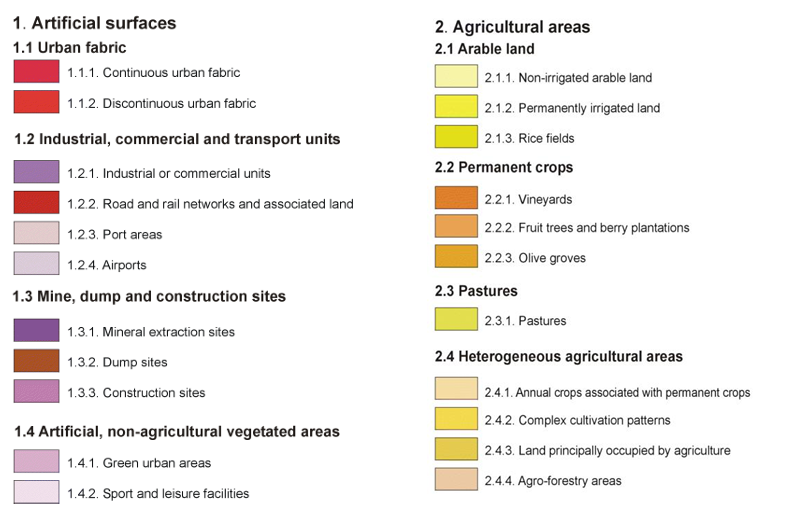
\includegraphics[width=0.5\linewidth]{Img/Theme/clc1.png}
    \caption[Ejemplo U-net]{Representación gráfica de una U-net y las capas utilizadas \cite{medium.com}}
    \label{fig:u-net}
\end{figure}